\graphicspath{{Kapitel/Kapitel1_Einleitung/Images/}}

Der Einsatz künstlicher Intelligenzen ist aktuell in allen Bereichen der Informatik auf dem Vormarsch. Dies gilt vor allem für die Automobilindustrie, da das Thema des autonomen Fahrens nicht ohne intelligente Algorithmen realisierbar ist. Eine wichtige Rolle bei der Entwicklung solcher Algorithmen spielt dabei das maschinelle Lernen. Dabei wird versucht, ausgehend von vielen lehrreichen Beispieldaten, die Lösung einer Aufgabe zu lernen und auf andere unbekannte Daten zu verallgemeinern. So kann ein System auch auf vorher ungesehene Daten reagieren, was mit einer statischen Programmierung nur schwer oder gar nicht möglich ist. Der Erfolg dieses Prinzips hängt genauso von der Qualität der Trainingsdaten ab wie der des Algorithmus. Deshalb wird in die Erstellung dieser Daten sehr viel Arbeit gesteckt.\\

Im Bereich der Fahrerassistenzsysteme und des autonomen Fahrens ist es wichtig, dass das Auto seine Umgebung so gut wie möglich wahrnehmen kann. Deshalb werden für Algorithmen, die in diesen Bereichen angewendet werden, Daten von Sensoren verwendet um das Umfeld des Autos wahrzunehmen. Dies sind meist Kamera-, Rader- oder Lidarsensoren. Die Eingangsdaten dieser Sensoren müssen nun so aufbereiten werden, damit ein lernendes Computersystem etwas damit anfangen kann. Dazu werden alle, für das Anwendungsfeld wichtigen Teile mit entsprechenden Klassifikationen versehen. Zum Beispiel werden auf einem Kamerabild alle Personen und Fahrzeuge als eben diese markiert, sodass das Fahrzeug  lernen kann wie Personen und Fahrzeuge aussehen und diese dann später im Straßenverkehr selbstständig erkennt. Radar- und Lidarsensoren liefern stattdessen Punktwolken als Eingangsdaten (vgl. Abbildung \ref{fig:Punktwolke}), das Prinzip bleibt allerdings das gleiche. Auch hier müssen alle wichtigen Teile, in diesem Fall Punkte, mit entsprechenden Klassen versehen werden. Dieser Vorgang nennt sich Labeln.\\

\begin{figure}%
	\centering
    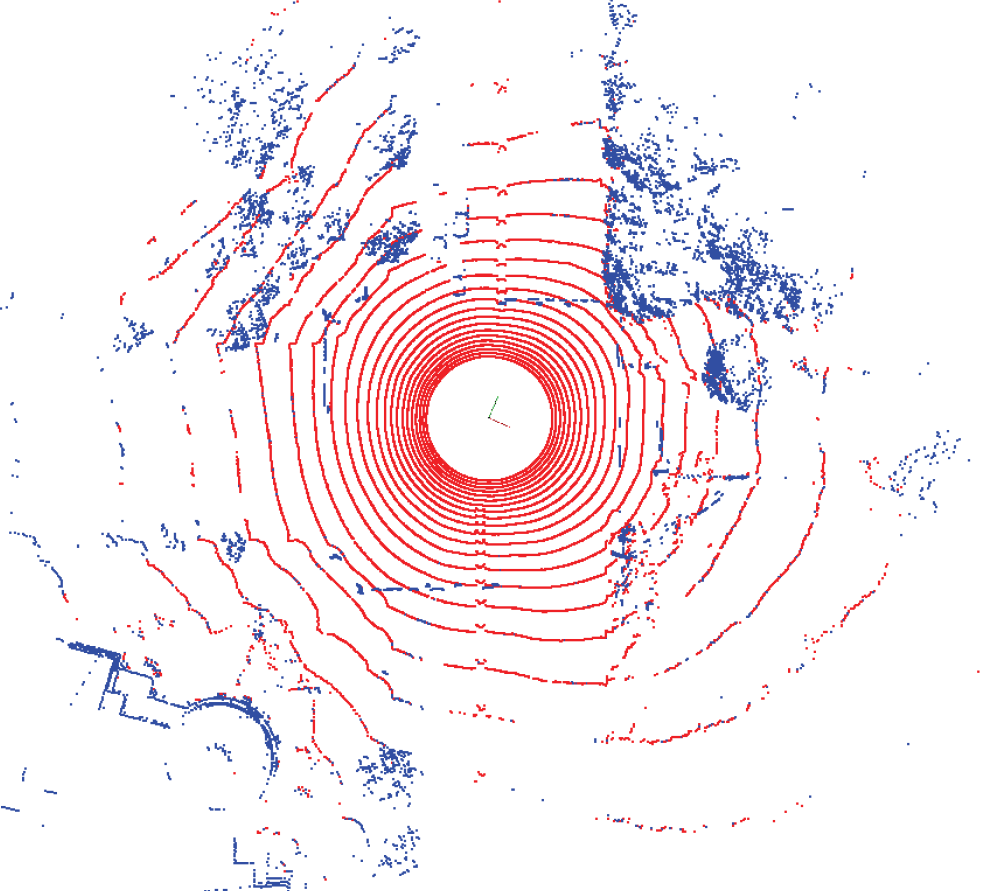
\includegraphics[width=7.5cm]{Punktwolke}\label{fig:Punktwolke}
    \caption{Vogelperspektive auf eine Lidar-Punktwolke, wobei dir roten Punkte alle Boden- und die blauen alle Nicht-Bodenpunkte darstellen}
\end{figure}


\section{Motivation}
In einem bislang aufwändigen Verfahren müssen diese Punktwolken so aufbereitet und mit einer Bedeutung versehen werden, dass die Algorithmen an diesen Beispielen lernen, Unterscheidungen und Erkennungen selbst durchführen zu können und dabei möglichst wenige Fehler machen. Dabei kommen aktuell Softwarewerkzeuge zum Einsatz welche die Sensordaten für einen menschlichen Benutzer visualisieren und dieser sie dann manuell mit unterschiedlichen Bedeutungen versehen kann. Wegen der großen Menge an Daten, die für das Trainieren der Algorithmen benötigt wird, muss dieses manuelle Annotieren möglichst effizient durchführbar sein.\\

Ein zweidimensionales Kamerabild kann sehr einfach auf einem Computermonitor dargestellt und bearbeitet werden. Eine besondere Herausforderung stellt jedoch die Verarbeitung von 3-D-Daten, wie einer Punktwolke, dar. Hier stößt man mit den Möglichkeiten eines zweidimensionalen Computermonitors schnell an die Grenzen einer effizienten Darstellung und Bearbeitung. So ist es beispielsweise für die Annotierung solcher Punktwolken und ihrer Einzelmesswerte schwierig, die optimale Perspektive auf die Daten zu finden, die eine effiziente Erfassung durch den Menschen und eine entsprechende Bearbeitung zulässt. Dies erfordert von den Benutzern sehr viel Übung und Erfahrung, durch entsprechende Drehungen der Punktwolkendarstellung sich in dieser zurechtzufinden und Messpunkte realen Objekten zuzuordnen.\\ 

Eine alternative dazu soll diese Masterarbeit bieten, welche eine Applikation beschreibt, die das Visualisieren und Annotieren von Punktwolken einfacher und effizienter gestaltet. Mittels neuartiger Technologien wie Virtual- und Augmented Reality soll die Grenze zwischen 2-D und 3-D aufgehoben werden, sodass man sich als interaktiver Teilnehmer im dreidimensionalen Raum durch die Sensordaten navigieren, mit ihnen interagieren und sie annotieren kann.\\

\section{Ziel der Arbeit}
Ziel dieser Arbeit ist es zunächst ein passendes Medium für eine solche Applikation zu finden, das nicht nur die Anforderungen der Applikation selbst erfüllt, sondern auch an einem handelsüblichen Büro-Arbeitsplatz verwendet werden kann. Anschließend soll eine Applikation erstellt werden die folgende Grundfunktionalität erfüllt:\\

\begin{enumerate}
\item Mit der Anwendung soll es Möglich sein ein, bei CMORE gängiges, Datenformat einzulesen und alle nötigen Informationen daraus zu extrahieren

\item Aus den extrahierten Informationen soll eine Punktwolke generiert und innerhalb des gewählten Mediums visualisiert werden.

\item Der Benutzer muss die Möglichkeit haben durch die Punktwolke zu navigieren.

\item Die Applikation muss die Möglichkeit bieten jeden einzelnen Punkt mit einer Klassifikation versehen zu können. Dabei sollen Alleinstellungsmerkmale des gewählten Mediums benutzt werden, um eine vorzeigbare Verbesserung gegenüber der herkömmlichen Computer-Monitor-Annotation zu generieren. 

\item Alle getätigten Annotationen müssen in die eingelesenen Dateien zurückgeschrieben bzw. in neue Dateien exportiert werden.
\end{enumerate}

Anschließend sollen die Basisfunktionen erweitert und zusätzliche Funktionen hinzugefügt werden. Abhängig von der verbleibenden Zeit soll die Anwendung gemäß folgender Priorität erweitert werden:\\

\begin{enumerate}
\item Es sollen neue Möglichkeiten zur Annotation von Punkten implementiert werden

\item Die Möglichkeit, eigene Klassifikationen für Punkte zu erstellen, soll 
\end{enumerate}

Am wichtigsten wäre hierbei die Applikation um effiziente Möglichkeiten zu erweitern um Punkte zu labeln. Außerdem sollte es für den Benutzer möglich sein individuelle Klassifikationen anzulegen, um unterschiedliche Anwendungsgebiete abzudecken. Optional sind neue Navigationsmöglichkeiten und einlesbare Datenformate. 




